%!TEX root = parita-msc.tex

\chapter{Related Work}
\label{chap:relwork}

\begin{doublespace}

This Chapter reviews the theoretical and practical work
on the semantic web and \ac{lod},
from the perspectives of technology and usability,			
that form the foundation of this thesis.

The web was first designed by Berners-Lee in 
1989\footnote{\tt https://www.w3.org/History/1989/proposal.html} 
while working at the \ac{cern}.
On the original web, of documents, 
the web pages were written and the links between 
pages were described using \ac{html}.
On the next web, of data, 
the web pages are written using \ac{html} and the relationships amongst
entities on those pages are described using \ac{rdf}.
These differences are illustrated in Figure~\ref{semantic-web}.

\begin{figure}[htp]
    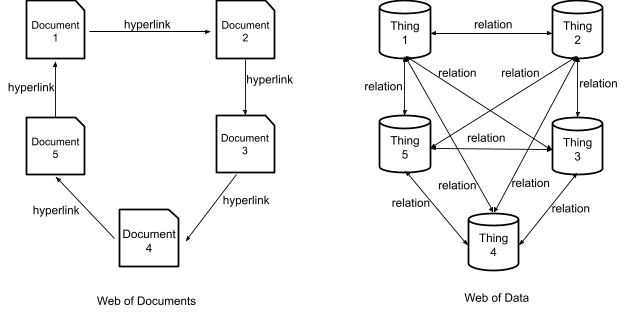
\includegraphics[width=\columnwidth]{images/ch2/semantic-web.png}
    \caption{Following Aghaei et al.~\cite{aghaei2012evolution},
    an illustration of the contrast between the web of documents
    that uses \ac{html} and the web of data that uses \ac{rdf}.
    \label{semantic-web}}
\end{figure}

\section{Linked Open Data}
\label{sec:linkedopendata}

Linked Open Data is the amalgamation of
linked data, that expresses the relationships between data,
and open data, that grants broad access rights to the data.
The relationships amongst data are equally important 
to the working of the semantic web 
as the access to the data itself~\cite{bizer2011linked}.

In 2006, 
Berners-Lee~\cite{bizer2009linked} 
described four basic rules 
for publishing and connecting 
structured datasets across the web. 
These rules have become known as the 
linked data 
principles, and have been enhanced by Berners-Lee, Bizer, Heath, 
and Idehen~\cite{bizer2009emerging, bizer2011linked, bizer2008linked, heath2011linked}.
Those rules are presented here. 
Terminology introduced in the rules is described in the subsequent text.

Rule 1.
Use \acp{uri} as unique names for (all) things on the web,
so that the same \ac{uri} used in different datasets is understood to signify
the same thing.

Rule 2.
Use \ac{https} (or \ac{http}) \acp{uri} to look up those unique names
because the hypertext transfer protocols allow easy retrieval of resources,
which promotes the publication and use of data on the web.

Rule 3.  
Provide useful information to others, using standards from the \ac{rdf} family,
in response to a look-up of a unique name associated with one of your \acp{uri}.
   
Rule 4.
Use other (existing) \acp{uri} in your data to encourage discovery of more relationships,
which promotes the global interconnection of data.

These principles encourage the
naming of subjects, predicates, and objects with 
\ac{https} \acp{uri}\footnote{\tt https://www.w3.org/TR/uri-clarification/} 
and providing useful information through the \ac{rdf} family of standards.
Berners-Lee introduced the concept of 5-star 
\ac{lod}\footnote{\tt https://www.w3.org/TR/ld-glossary/\#x5-star-linked-open-data}
to denote structured data on the web as \ac{rdf} wherein all identifiers are \ac{https} \acp{uri}
pointing to other useful data sources, with an open license for access.

\subsection{Uniform Resource Identifiers}
\label{subsec:uri}

Resources on the web, 
whether they are abstract (logical) or physical,
are identified by a unique string of ASCII characters known 
as a \ac{uri}.
As described by Berners-Lee et al.~\cite{RFC3986uri} 
in RFC 3986 (which became STD 66), 
this unique string is subject to guidelines and security considerations 
while defining the syntax for a generic \ac{uri} 
and a process for resolving \ac{uri} references. 
Berners-Lee et al.~\cite{RFC3986uri} 
characterized \ac{uri} by discussing the component terms.

Numerous advantages come from uniformity. 
Various types of resource identifier can be used
in the same context even when the means accessing those resources may vary. 
Semantic interpretation of standard syntactic rules is the same
across various types of resource identifiers. 
New types of resource identifiers can be introduced
without affecting how other identifiers are used. 
Existing resource identifiers can be reused in a variety of settings, 
enabling new applications or protocols to benefit from that 
widely-utilized set of resource identifiers.

A resource is anything that can be identified
by a \ac{uri}. The pages on a website are a recognizable example. 
A resource is not necessarily available via the web. 
It may correspond to a physical entity such as a person,
an abstract concept such as a relationship,
or a numeric quantity.

An identifier distinguishes an object from all other objects within its scope.
The purpose of an identifier is to distinguish one resource from all others.
An identifier is not required to define the identity of what is referenced, 
though this may be the true for some.
A system using \acp{uri} is neither required to access the resource identified
and for some there is no intention that they be accessed.
    
Berners-Lee et al.~\cite{RFC3986uri} defined the generic syntax of a \ac{uri} 
as shown in Figure~\ref{syntax-diagram}. 
A \ac{uri} comprises five components in sequence 
(see Examples~\ref{generic-uri} and~\ref{authority-uri}). 
It is not mandatory for a \ac{uri} to have all the components.
\begin{flalign}
    \text{\tt \ac{uri} = scheme: [//authority] path [?query] [\#fragment]} &&
    \label{generic-uri}
\end{flalign}
\noindent
The authority component comprises three elements, which are:
\begin{flalign}
    \text{\tt authority = [userinfo@] host [:port]} &&
    \label{authority-uri}
\end{flalign}

\begin{figure}[h]
    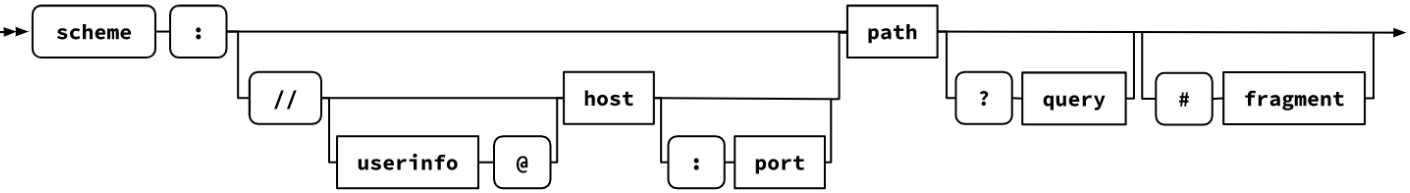
\includegraphics[width=\columnwidth]{images/ch2/syntax-diagram.png}
    \caption{Syntax diagram for a generic \ac{uri}, 
    after Berners-Lee et al.~\cite{RFC3986uri}.}
    \label{syntax-diagram}
\end{figure}
\noindent
One of the \acp{uri} from the Survey ontology is in Example~\ref{example-uri}.
Figure~\ref{components-of-uri-example} 
shows its components.
\begin{flalign}
    \text{\tt https://parita-amin.github.io/survey.owl\#Survey} &&
    \label{example-uri}
\end{flalign}

\begin{figure}[ht]
    \centering
    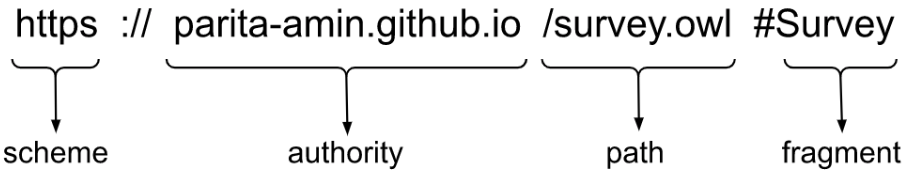
\includegraphics[width=\columnwidth]{images/ch2/components-of-uri-example.png}
    \caption{Components of the example \ac{uri}, 
    after Berners-Lee et al.~\cite{RFC3986uri}}
    \label{components-of-uri-example}
\end{figure}

\subsection{Resource Description Framework}
\label{subsec:rdf}

According to Flanders and Jannidis~\cite{julia2015data}, 
data modelling refers ``the process of representing data, 
their relationships, and their semantics in a way 
which is processable by humans and machines''. 
A data model is 
an abstract representation of data 
that standardizes how its components 
relate to one another and to the characteristics of real-world objects. 
Depending on the level of abstraction, 
there are three main types of data models, 
namely, 
conceptual, logical, and physical data model. 
Some widely-used primary data models are 
dimensional, relational, and \ac{er} models. 
RDF began as a metadata model and is now the means to describe resources 
(entities) and the relationships amongst them in a computer-understandable format, 
using basic data models like the \ac{er} model. 
An \ac{er} model is a high-level conceptual data model 
that assists rigorous analysis of the data requirements 
to build a well-designed database. 
The \ac{er} model depicts real-world entities and the relationships between them~\cite{lin2019structure}.

\ac{rdf} uses {\em properties} and {\em property values} 
to describe resources, which are named by \acp{uri}. 
The three types of objects in \ac{rdf} are resources, properties, and statements.
Each data object in a dataset on the web is considered a resource and is named 
using a \ac{uri}. 
The resources available on the web must be named using \ac{https} \acp{uri}. 
The \ac{w3c} has defined the 
{\tt rdf:type} 
property to represent the 
``object of one or more classes''~\cite{cyganiak2014rdf}. 
Resources are described by their characteristics, 
called {\em properties}. 
The object of \ac{rdf} 
that is used to combine a resource with a property of its value is a {\em statement}. 
A statement, 
in general terms, 
can be seen as building blocks of a statement in English, 
which are a subject, a predicate, and an object. 
An object in a statement can be either a property value, a resource, or a literal. 
\ac{rdf}, 
according to Beckett, Gandon and Schreiber~\cite{gandon2014rdf,zongmin2016rdf}, 
can be represented in three ways:
using \ac{xml} in an \ac{rdf}/\ac{xml} document,
as triples in subject-predicate-object form 
or in graphical form.

The University of Manchester has developed Pizza ontology 
which acts as an inspiration for ``pizza'' examples in this chapter.
Consider the following example:
\begin{flalign}  
    \text{\tt Pizza has CaloricContent with some integer value}&&
    \label{caloriccontent}
\end{flalign}
\noindent
Figure~\ref{rdf-xml-doc} shows the \ac{rdf}/\ac{xml},
which consists of various \ac{xml} tags.
An \ac{rdf}/\ac{xml} 
document starts and ends with {\tt <rdf:\ac{rdf}>} and 
{\tt </rdf:\ac{rdf}>} respectively.
    
\begin{figure}[h]
	\framebox{\vbox{\tt\small
        \begin{tabbing}
            \hspace*{0.5cm}\=\hspace*{0.5cm}\=\hspace*{0.5cm}\=\hspace*{0.5cm}\= \kill
            \hspace*{\columnwidth}\\[-1cm]
            @prefix rdf: <http://www.w3.org/1999/02/22-rdf-syntax-ns\#> .\\
            @prefix owl: <http://www.w3.org/2002/07/owl\#> .\\
            @prefix pizza: <http://www.semanticweb.org/pizzatutorial/ontologies/2020/ \\ \>\>\> PizzaTutorial\#> .\\
            @prefix xsd:  <http://www.w3.org/2001/XMLSchema\#> .\\
            <rdf:RDF>\\
            \><owl:Class rdf:about="pizza:Pizza">\\
            \>\>\><owl:onProperty rdf:resource="pizza:hasCaloricContent"/>\\
            \>\>\><owl:someValuesFrom rdf:resource="xsd:integer"/>\\
            \></owl:Class>\\
            </rdf:RDF>
            \\[-1cm]
        \end{tabbing}
      }}
      \caption{Example~\ref{caloriccontent} expressed as \ac{rdf}/\ac{xml}.}
      \label{rdf-xml-doc}
\end{figure}
     
{\tt http://www.semanticweb.org/pizzatutorial/ontologies/2020/PizzaTutorial\#},  
{\tt http://www.w3.org/1999/02/22-rdf-syntax-ns\#},  
{\tt http://www.w3.org/2002/07/owl\#}, and 
{\tt http://www.w3.org/2001/XMLSchema\#}
are the base \acp{uri} that have been expressed using prefixes 
{\tt pizza}, {\tt rdf}, {\tt owl}, and {\tt xsd} respectively 
for the classes and properties in Figure~\ref{rdf-xml-doc}. 
The resource being described is {\tt pizza:Pizza}, 
{\tt pizza:hasCaloricContent} is the property, and 
{\tt xsd:integer} is the value.

Figure~\ref{rdf-triple} 
shows an example of an \ac{rdf} triple, 
where {\tt pizza:Pizza} is the subject; 
the predicate is {\tt pizza:hasCaloricContent}; 
and the object is {\tt xsd:integer}. 

\begin{figure}[htp]
    \framebox{\vbox{\tt\small
    \begin{tabbing}
        \hspace*{0.9cm}\=\hspace*{0.9cm}\=\hspace*{0.9cm}\=\hspace*{0.5cm}\= \kill
        \hspace*{\columnwidth}\\[-1cm]
        Subject: {\tt pizza:Pizza}\\
        \>\>Predicate: {\tt pizza:hasCaloricContent}\\
        \>\>\>\>Object: {\tt xsd:integer}
        \\[-1cm]
    \end{tabbing}
    }}
    \caption{An illustration of Example~\ref{caloriccontent} as an \ac{rdf} triple.}
    \label{rdf-triple}
\end{figure}
  
Figure~\ref{rdf-graph} 
shows Example~\ref{caloriccontent} in graphical format. 
A resource is represented by an oval;
a property value is represented by a rectangle;
and a property is represented by an arrow,
to show that the property (predicate, {\tt pizza:hasCaloricContent}) 
connects the resource (subject, {\tt pizza:Pizza}) with the value (object, {\tt xsd:integer}).
    
\begin{figure}[htp]
    \centering
    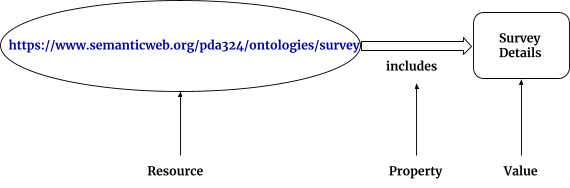
\includegraphics[width=\columnwidth]{images/ch2/rdf-graph.png}
    \caption{Graphical representation of Example~\ref{caloriccontent}.}
    \label{rdf-graph}
\end{figure}
    
The subject and object of an \ac{rdf} triple of \ac{rdf} act as nodes in the graph
where they are two entities and 
the predicate being the third entity acts as a connector between them. 
Considering an entity-relationship data model, 
the predicate can be treated as a relationship shared by the subject and the object. 
In addition to the \ac{rdf}/\ac{xml} and the line-based N-triples~\cite{beckett2014rdf} 
formats, 
the \ac{rdf} data model has a variety of serialization formats such as
\ac{turtle}; \ac{n3}, 
which is an extension of N-Triples (line based) 
and adds a graph label to each line 
that allows multiple graph encoding~\cite{cyganiak2008n}.

There can be more details added to Example~\ref{caloriccontent}
(illustrated in Figures~\ref{rdf-xml-doc},~\ref{rdf-triple}, and~\ref{rdf-graph}). 
That is, 
more statements can be added in relation to the original statement.  
Suppose the new statement added is: 
\begin{flalign}  
    \text{\tt Pizza has PizzaBase} &&
    \label{pizzabase}
\end{flalign}
\noindent
where the property (predicate, {\tt pizza:hasBase}) 
connects the resource (subject, {\tt pizza:Pizza}) with the value (object, {\tt pizza:PizzaBase}).
Figure~\ref{graph-for-relative-statements} shows a graphical representation
of the two example statements combined.

\begin{figure}[ht]
    \centering
    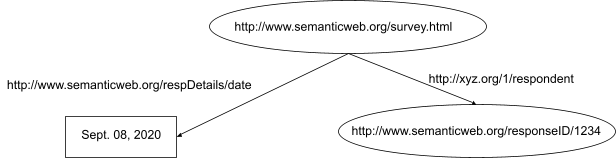
\includegraphics[width=\columnwidth]{images/ch2/graph-for-relative-statements.png}
    \caption{Graphical representation of Examples~\ref{caloriccontent} and~\ref{pizzabase} combined,
    following the \ac{rdf} Primer~\cite{manola2004rdf}.}
    \label{graph-for-relative-statements}
\end{figure}
\noindent
Adding more complexity to the system,
include a description of the types of {\tt PizzaBase}.
Figure~\ref{graph-for-base-types} 
shows a graphical representation of this system.
\begin{flalign}  
    \text{ {\tt DeepPanBase} and {\tt ThinAndCrispyBase}} &&
    \label{kindsofbase}
\end{flalign}

\begin{figure}[ht]
    \centering
    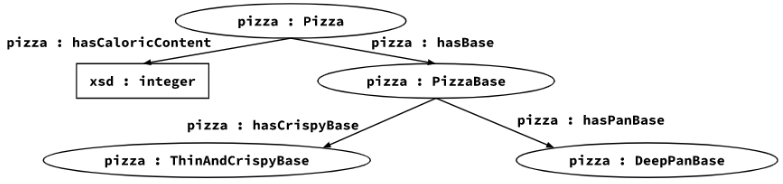
\includegraphics[width=\columnwidth]{images/ch2/graph-for-base-types.png}
    \caption{Graphical Representation of \ac{rdf} with types of PizzaBase, 
    after the \ac{rdf} Primer~\cite{manola2004rdf}.}
    \label{graph-for-base-types}
\end{figure}

{\tt pizza:Pizza} (subject) 
is connected to {\tt pizza:PizzaBase} (object) node 
through {\tt pizza:hasBase} (predicate). 
Further, 
the {\tt pizza:PizzaBase} node has multiple child nodes, 
namely, 
{\tt pizza:ThinAndCrispyBase} and {\tt pizza:DeepPanBase} 
where the \acp{uri} for the predicates are 
{\tt pizza:hasCrispyBase} and {\tt pizza:hasPanBase} respectively. 
Instead of using an unnecessary \ac{uri} 
for the {\tt pizza:PizzaBase} entity, 
a blank node can be used to denote the entity, 
as shown in Figure~\ref{blank-node-for-rdf}. 
As the relationships of the node with other nodes give sufficient details without hindering the flow of the data tree, 
the node does not require a 
\ac{uri} reference.

\begin{figure}[htp]
    \centering
    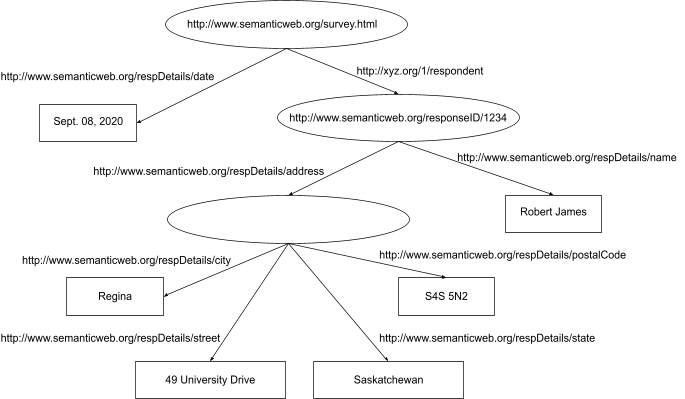
\includegraphics[width=\columnwidth]{images/ch2/blank-node-for-rdf.png}
    \caption{\ac{rdf} Representation in Figure~\ref{graph-for-base-types} 
    without a \ac{uri} (blank node) for PizzaBase Entity, after the \ac{rdf} 
    Primer~\cite{manola2004rdf}.}
    \label{blank-node-for-rdf}
\end{figure}

According to the \ac{w3c} 
Recommendation\footnote{\tt https://www.w3.org/TR/rdf11-concepts/},  
the design should 
``have a simple data model; 
formal semantics and provable inference; 
should use an extensible \ac{uri}-based vocabulary and an \ac{xml}-based syntax; 
should support the use of \ac{xml} schema datatypes; 
and should allow any one to make statements about any resource''. 

\ac{rdfs}, 
according to McBride~\cite{mcbride2004resource}, 
was introduced by the \ac{w3c} 
as a technique to define resource types and property names. 
The data publishers can use \ac{rdfs} 
to define various vocabularies in an \ac{rdf} model. 
Some of the commonly used \ac{rdfs} classes and properties\footnote{\tt https://www.w3.org/TR/rdf-schema/} 
along with their description are listed in Table~\ref{rdfs-classes-and-properties}~\cite{mcbride2004resource}.

\begin{table}[h!]
	\centering
    \begin{tabular}{| l | p{10cm} |} \hline
		Class/Property & Description  \\  \hline
     rdfs:Resource & All things described by \ac{rdf} are called resources  \\ \hline
     rdfs:Class & The class of resources that are \ac{rdf} classes \\ \hline
     rdf:Property & The class of \ac{rdf} properties. 
     It is an instance of rdfs:Class  \\ \hline
     rdfs:Literal & The class of literal values like integers and strings  \\ \hline
     rdfs:Datatype & The class of datatypes. All the objects of this class correspond to the \ac{rdf} model of datatype  \\ \hline
     rdf:HTML & The class of \ac{html} literal values and subclass of rdfs:Literal  \\ \hline
     rdfs:range & An instance of rdf:Property that is used to state that the values of a property are instances of one or more classes \\ \hline
     rdfs:domain & An instance of rdf:Property that is used to state that any resource that has a given property is an instance of one or more classes \\ \hline
     rdf:type & An instance of rdf:Property that is used to state that a resource is an instance of a class  \\ \hline
     rdfs:subClassOf & An instance of rdf:Property that is used to state that all the instances of one class are instances of another  \\ \hline
     rdfs:label & an instance of rdf:Property that may be used to provide a human-readable version of a resource's name  \\ \hline
     rdfs:subPropertyOf \ \ & An instance of rdf:Property that is used to state that all resources related by one property are also related by another  \\ \hline
    \end{tabular}
    \caption{Commonly used Classes and Properties of RDFS}
    \label{rdfs-classes-and-properties}
\end{table}

\subsection{Open Data}
\label{subsec:opendata}

According to the Open Knowledge Foundation~\cite{foundation}, 
``Open Data is data that can be freely used, 
re-used and redistributed by anyone - subject only, 
at most, 
to the requirement to attribute and share-alike''. 
To make open data available to everyone on the web, 
the data don't need to be interlinked. 
Important features of open data are:

\begin{itemize}

	\item Availability and access: 
	the data should be available on the web. 
  	The users should be able to access the data easily by downloading 
	them over the internet.
	It should be easy to access and modify the data.
  
  	\item Re-use and redistribution: 
	the data on the web must have permissions to re-use and 
	redistribute in combination to other datasets.
 
	\item Universal participation: 
	the data should be available to use, re-use, 
	and redistribute for all the users without any 
	discrimination to an individual or a group.
	
\end{itemize}

Linked data is concerned with publishing structured data,
along with the semantics of the relationships amongst that data,
onto the web.
The \ac{w3c} standards and technologies handle the distribution and 
engagement of this data across the web with the potential to present 
it as one huge database~\cite{bernerslee1999weaving}.

\subsection{Wikidata}
\label{subsec:wikidata}

A variety of projects and websites, 
that use linked open data, 
have been developed. 
Wikidata is one of the major projects of linked open data that present structured data on the semantic web. 

Krotzsch and Vrandecic~\cite{denny2014wikidata}
describe the introduction of Wikidata to the world in 2012. 
According to Erxleben et al.~\cite{fredo2014intro}, 
Wikidata is ``the community-created knowledge base of Wikipedia 
and the central data management platform for Wikipedia''. 
It was established for the collection and integration of Wikipedia data  
into
the semantic web. 
Wikidata is a free and open-source tool that handles a large amount of 
structured data and maintains pages that store the data. 
Each entity on Wikidata represents the subject of a triple with a dedicated page. 
The properties of Wikidata are similar to that of \ac{rdf} 
where the individuals and classes are indicated using items. 
Data on a page of the Wikidata is available for the users to access as well as edit.

For instance, 
the University of Regina (Q3104287) 
has an item page\footnote{\tt https://www.wikidata.org/wiki/Q3104287}.
Figure~\ref{wikidata-uofr} 
illustrates a portion of the contents of this page. 

\begin{figure}[htp]
    \centering
    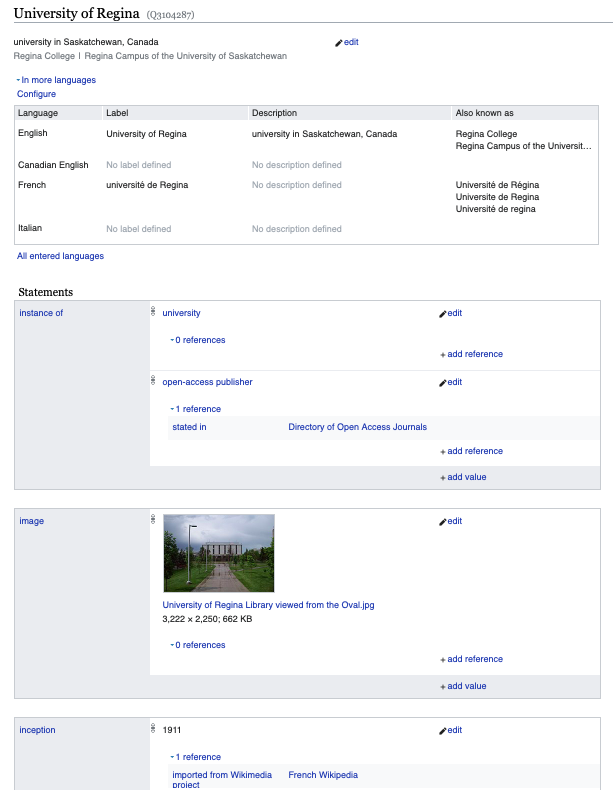
\includegraphics[width=\columnwidth]{images/ch2/wikidata-uofr.png}
    \caption{A portion of the item page for ``University of Regina'' on Wikidata.}
    \label{wikidata-uofr}
\end{figure}

Wikidata uses a method of automatically assigning unique identifiers to the entities, 
which are used as the labels of the item pages instead of the actual names of the entities. 
These identifiers are a string starting with a capital Q followed by a sequence of digits. 
The identifiers are assigned irrespective of the language as the Wikidata website supports multiple languages.

An item page on Wikidata consists of two main sections.
The first section, entitled Statements, contains a list properties and values.
The properties, along with their property IDs, used for the University of Regina 
are listed in Table~\ref{uofr-statement-properties-and-id}.
The other section is Identifiers, which consists of various IDs associated with the subject.
The identifiers, along with their property IDs, used for the University of Regina 
are listed in Table~\ref{uofr-identifier-properties-and-id} 
where as the \ac{rdf}/\ac{xml} 
description of the University of Regina on Wikidata is as shown in Figure~\ref{rdf-xml-uofr}. 
  
\begin{table}[h!]
        \centering
        \begin{tabular}{|l|l|} \hline 
             Statement Property \ & Property ID \\ \hline
             instance of & P31\\ \hline
             image & P18\\ \hline
             inception & P571\\ \hline
             country & P17\\ \hline
             located in the administrative territorial entity & P131\\ \hline
             coordinate location & P625\\ \hline
             subsidiary & P355\\ \hline
             official website & P856\\ \hline
             commons category & P373\\ \hline
             topic's main category & P910\\ \hline
             category for employees of the organization & P4195\\ \hline
             category for alumni of educational institution & P3876\\ \hline
             API endpoint & P6269\\ \hline
             social media followers & P8687\\ \hline
        \end{tabular}
        \caption{Statement Properties and Property IDs for ``University of Regina'' on Wikidata.}
        \label{uofr-statement-properties-and-id}
\end{table}
   
\begin{table}[h!]
	\centering
  	\begin{tabular}{|l|l|} \hline
	Identifier Property \ & Property ID \\ \hline
    VIAF ID & P214\\ \hline
    ISNI & P213\\ \hline
    GND ID & P227\\ \hline
    Library of Congress authority ID & P244\\ \hline
             WorldCat Identities & P7859\\ \hline
             ARWU university ID & P5242\\ \hline
             Crossref funder ID & P3153\\ \hline
             Facebook ID & P2013\\ \hline
             Freebase ID & P646\\ \hline
             Google Maps Customer ID & P3749\\ \hline
             GRID ID & P2427\\ \hline
             HAL structure ID & P6773\\ \hline
             LittleSis organization ID & P3393\\ \hline
             Microsoft Academic ID & P6366\\ \hline
             Ringgold ID & P3500\\ \hline
             ROR ID & P6782\\ \hline
             Times Higher Education World University ID & P5586\\ \hline
             Twitter username & P2002\\ \hline
             U-Multirank university ID & P5600\\ \hline
	\end{tabular}
    \caption{Identifier Properties and Property IDs for ``University of Regina'' on Wikidata.}
    \label{uofr-identifier-properties-and-id}
 \end{table}

\begin{figure}[htp]
    \framebox{\vbox{\tt\small
    \begin{tabbing}
        \hspace*{0.9cm}\=\hspace*{0.9cm}\=\hspace*{0.9cm}\=\hspace*{0.5cm}\= \kill
        \hspace*{\columnwidth}\\[-1cm]
        <?xml version="1.0" encoding="utf-8" ?>\\
        <rdf:RDF xmlns:rdf="http://www.w3.org/1999/02/22-rdf-syntax-ns\#"\\
        \>xmlns:xsd="http://www.w3.org/2001/XMLSchema\#"\\
        \>xmlns:ontolex="http://www.w3.org/ns/lemon/ontolex\#"\\
        \>xmlns:wdt="http://www.wikidata.org/prop/direct/"\\
        \>xmlns:wdtn="http://www.wikidata.org/prop/direct-normalized/">\\
        <rdf:Description rdf:about="https://www.wikidata.org/wiki/Special:EntityData/Q3104287">\\
        \><rdf:type rdf:resource="http://schema.org/Dataset"/>\\
        \><schema:about rdf:resource="https://www.wikidata.org/entity/Q3104287"/>\\
        \><cc:license rdf:resource="http://creativecommons.org/publicdomain/zero/1.0/"/>\\
        \><rdf:Description rdf:about="https://en.wikipedia.org/wiki/University\_of\_Regina">\\
        \>\><rdf:type rdf:resource="http://schema.org/Article"/>\\
        \>\><schema:about rdf:resource="http://www.wikidata.org/entity/Q3104287"/>\\
        \>\><schema:inLanguage>en</scehma:inLanguage>\\
        \>\><schema:isPartOf rdf:resource="https://en.wikipedia.org/"/>\\
        \>\><schema:name xml:lang="en">Univeristy of Regina</schema:name>\\
        \>\><schema:description xml:lang="en">university in Saskatchewan, Canada\\\>\></schema:description>\\
        \>\><wdt:P18 rdf:resource="http://commons.wikinedia.org/wiki/Special:FilePath/\\ \>\>University\%20of\%20Regina\%20Library\%20viewed\%20from\%20the\%20Oval.jpg"/>\\
        \></rdf:Description>\\
        </rdf:Description>\\
        </rdf:RDF>
        \\[-1cm]
    \end{tabbing}
    }}
    \caption{Wikidata Entry (RDF/XML) for ``University of Regina''.}
    \label{rdf-xml-uofr}
\end{figure}

\section{Ontology in Web Semantics}
\label{sec:ontologyinwebsemantics}

Ontology is a branch of information science 
that encloses representation, nomenclature, and 
definition of various properties, categories, and relationships shared among 
entities, which includes all types of data, concepts and entities,
that support any number of domains 
in which the user is interested.
In other words, 
ontology is a form of defining a set of concepts for representing the subject 
properties and the relationships shared among them. 
According to Gruber~\cite{gruber1995towards}, 
ontology is 
{\tt an explicit specification of a conceptualization}, 
where conceptualization is 
``an abstract, simplified view of the world 
(includes objects, concepts and other entities 
that are assumed to exist in some area of interest and the relationships 
that hold among them) 
that we wish to represent for some purpose''. 
In web semantics, 
an ontology is used to define the semantics of the resources briefly and methodically. 
On the semantic web, 
the ontologies have been used 
to define resources' conceptual and physical qualities 
in the form of metadata schema for a predetermined group of users.

\subsection{OWL Ontologies}
\label{subsec:owlontologies}

The \ac{w3c} developed a standard ontology language called 
\ac{owl}\footnote{\tt https://www.w3.org/TR/owl-overview/} 
to define and describe concepts for ontology
using different facilities and operations like intersection, union and negation. 
It is based on a logical model 
on which a reasoner 
can be used to check the mutual consistency 
among the statements and definitions in the ontology. 
The reasoner is also responsible for the identification of a 
suitable concept for particular definitions~\cite{horridge2009practical}.

\subsection{Components of OWL Ontologies}
\label{subsec:componentsofowlontologies}

An \ac{owl} ontology consists of a set of components that define and describe the concepts collectively. 
The basic components of any \ac{owl} ontology, 
Individuals, Properties and Classes, 
are briefly explained in this section.

\subsubsection{Individuals}
\label{subsubsec:individuals}

According to Horridge et al.~\cite{horridge2009practical}, 
``Individuals represent objects in the domain in which we are interested''. 
Individuals are the objects of classes. 
Figure~\ref{owl-individuals} 
shows the representation of different individuals in various domains. 
The triangles are used here to denote the individuals in free space.

\begin{figure}[htp]
    \centering
    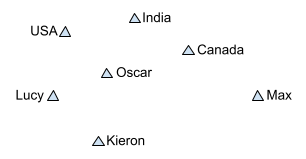
\includegraphics[width=8cm]{images/ch2/owl-individuals.png}
    \caption{Representation of Individuals in OWL}
    \label{owl-individuals}
\end{figure}

\subsubsection{Properties}
\label{subsubsec:properties}

Binary relationships, links shared by two individuals (things),
are called properties. 
For instance, 
the individuals 
{\tt Customer1} and {\tt AmericanaPizza1} from Figure~\ref{owl-individuals} 
are linked to each other by the property {\tt purchasedPizza}. 
Each property can have its inverse. 
For instance, 
{\tt purchasedPizza} 
can have an inverse property {\tt purchasedBy}. 
The properties can be symmetric or transitive. 
It is possible to have functional properties where the properties can be restricted to having only one value.

Figure~\ref{owl-properties} 
shows representation of properties between the individuals {\tt Customer1} and {\tt Medium}, 
and {\tt Customer1} and {\tt AmericanaPizza1}. 
The relation between {\tt Customer1} and {\tt Medium} is {\tt hasSpicinessPreference}. 
The arrow between two individuals in the figure denotes the property (relationship) between them.

\begin{figure}[htp]
    \centering
    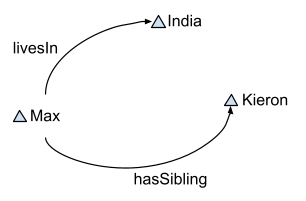
\includegraphics[width=8cm]{images/ch2/owl-properties.png}
    \caption{Representation of Properties in OWL}
    \label{owl-properties}
\end{figure}

\subsubsection{Classes}
\label{subsubsec:classes}

In \ac{owl}, 
the sets consisting of individuals are called \ac{owl} classes. 
Mathematical (formal) descriptions are used to describe the \ac{owl} classes. 
These descriptions include accurate statements on the requirements for the class membership. 
For instance, 
the class {\tt Customer} 
consists of all the individuals that are customers in the Domain of Discourse 
which can contain one or more classes. 
Inheritance in \ac{owl} classes (Class Hierarchy) 
may exist with the classes having subclasses and/or super-classes which is technically termed as taxonomy. 
``Subclasses specialise (``are subsumed by'') their super-classes''~\cite{horridge2009practical}. 
For instance, 
consider the classes {\tt Person} and {\tt Customer} from the pizza ontology, 
where {\tt Customer} is a subclass of {\tt Person}.
This implies the following statements:

\begin{itemize}

    \item All customers are person
    
    \item All members of class {\tt Customer} are members of class {\tt Person}
    
    \item Being a {\tt Customer} implies that individual is {\tt Person}
    
    \item {\tt Customer} is subsumed by {\tt Person}
    
\end{itemize}

Figure~\ref{owl-classes-with-individuals-and-properties} 
shows the representation of the classes 
for the individuals and properties that are 
shown in Figure~\ref{owl-properties}.

\begin{figure}[htp]
    \centering
    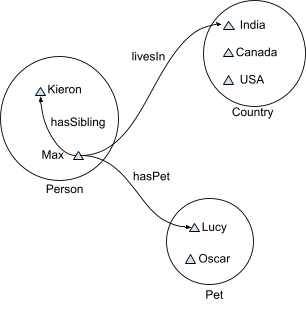
\includegraphics[width=8cm]{images/ch2/owl-classes-with-individuals-and-properties.png}
    \caption{Representation of OWL Classes Consisting of Individuals and Properties}
    \label{owl-classes-with-individuals-and-properties}
\end{figure}

\subsection{Ontology Editors}
\label{subsec:ontologyeditors}

Ontology editors are used by publishers 
to create new ontologies 
when the existing vocabulary is not suitable for their purpose. 
A list of ontology editors\footnote{\tt https://www.w3.org/wiki/Ontology\_editors} 
that can be used to edit, manage, organize and visualize ontology 
includes Protégé, NeOn Toolkit, SWOOP, Neologism, TopBraid Composer, 
Vitro, Knoodl, Anzo for Excel, OWLGrEd, Fluent Editor, Semantic Turkey, VocBench. 
Protégé is the most popular ontology editor among researchers. 
Most of the editors from the list are 
either non-existent or 
there exists negligible information about them, 
which has driven the decision of the use of protégé 
for ontology development which is discussed in detail in Chapter~\ref{chap:proofOfConcept}.

\section{Linked Data Life Cycle}
\label{sec:linkeddatalifecycle}

The Linked Data Life Cycle includes multiple stages as described by 
Ngomo et al.~\cite{ngomo2014introduction} 
which are listed in
Table~\ref{ldlc-stages}.
Each stage of this life cycle is independent yet linked to one another. 
So, 
it is not mandatory to go through all the stages sequentially 
to publish the data on the web. 
It is necessary to use a procedure that follows the life cycle 
to ensure the quality of data to be published as linked data. 
The first stage, 
generally, 
is data extraction along with conversion of the extracted data 
(in forms other than \ac{rdf}) into \ac{rdf}. 
Once the data is in \ac{rdf} form, 
any or all of the other stages listed in 
Table~\ref{ldlc-stages} 
can be performed.

\begin{table}[h!]
    \centering
    \begin{tabular}{|l|p{10cm}|} \hline 
     Stage & Description \\ \hline
     Extraction & Extraction and conversion of unstructured and semi-structured data into \ac{rdf}\\ \hline
     Storage \& Querying & Storing the \ac{rdf} data in a format that supports data querying efficiently\\ \hline
     Authoring & Allowing the users to create new data or to access and 
     modify the existing data\\ \hline
     Linking & Creating links among the data belonging to various domains and users based on their entities\\ \hline
     Enrichment & Data enrichment for efficient query support using various top-tier structures\\ \hline
     Quality Analysis & Managing data using different strategies to ensure good quality of available data on the web\\ \hline
     Browsing \& Exploration & Making the structured data available on the web for the users to browse and explore effectively\\ \hline
    \end{tabular}
    \caption{Stages in Linked Data Life Cycle, after Ngomo et al.~\cite{ngomo2014introduction}}
    \label{ldlc-stages}
\end{table}

The linked data life cycle is too basic and generic 
and may not be the best approach for describing data semantics. 
While working on this research, 
it was established that the life cycle~\cite{ngomo2014introduction} 
has gaps and does not aid the development of 5-star \ac{lov}.
Hence, this thesis introduces a new approach in Chapter~\ref{chap:methodology} 
that can be followed for developing \ac{lov} to map CSV data.

\section{Conversion of Data from Spreadsheets to RDF}
\label{sec:csvtordf}

The preferred format of the data published on the semantic web is \ac{rdf} format. 
Many data scientists use tables and spreadsheets to store and publish data using CSV
files over \ac{rdf} format 
as conversion of data to \ac{rdf} 
is comparatively difficult. 
The data used by Dr. Hepting has been stored in tabular format which can be converted into \ac{rdf} 
using different open source tools~\cite{ermilov2013csv} 
listed by \ac{w3c}\footnote{\tt https://www.w3.org/wiki/ConverterToRdf} 
or using \ac{rml}\footnote{\tt https://d2s.semanticscience.org/docs/convert-rml/}. 

\subsection{Tools to Describe CSV Data using Vocabulary}
\label{subsec:tools}

%Some of the open-source tools listed by the \ac{w3c} 
%for the mapping of CSV data using \ac{lov} are
%OpenRefine, RDF123, csv2rdf4lod, XLWrap, and Tarql.
%After an extensive research on these tools, 
%OpenRefine has been used in this thesis as most of these tools are out-dated.

%\subsubsection{OpenRefine}
%\label{subsubsec:openrefine}
%
%OpenRefine\footnote{\tt https://openrefine.org}, 
%an \ac{rdf} extension of Google Refine, 
%is a Java-based set of tools that work with messy data using \ac{grel}
%It allows the users to extract, transform, export, and convert 
%CSV, Excel, spreadsheets and other tabular data into \ac{rdf} 
%where a GUI (Graphical User Interface) is used to define schema mapping. 

\begin{itemize}
   
    \item OpenRefine:
    
    OpenRefine\footnote{\tt https://openrefine.org}, 
    an \ac{rdf} extension of Google Refine, 
    is a Java-based set of tools that work with messy data using \ac{grel}
    It allows the users to extract, transform, export, and convert 
    CSV, Excel, spreadsheets and other tabular data into \ac{rdf} 
    where a GUI (Graphical User Interface) is used to define schema mapping. 
   
    \item RDF123:
    
    RDF123\footnote{\tt https://ebiquity.umbc.edu/resource/html/id/237/RDF123-java-application-v1-0} 
    is a Java application and servlet for the conversion of CSV 
    and spreadsheets to \ac{rdf} 
    which uses arbitrary graphs to define schema mapping. 
    According to Han et al.~\cite{han2008rdf}, 
    it uses a graphical RDF123 template to allow users to convert the data from spreadsheets to \ac{rdf}.
   
    \item csv2rdf4lod:
   
    csv2rdf4lod\footnote{\tt https://github.com/timrdf/csv2rdf4lod-automation/wiki} 
    is a tool that is used for the conversion of tabular data into structured and linked \ac{rdf} 
    using specifications that are based on declarative \ac{rdf} 
    enhancement parameters. 
    It forms default namespaces for \acp{uri} 
    and provides VoID and original metada for the conversion 
    using identifiers for source organization, dataset and version.
   
    \item XLWrap:
    
    XLWrap\footnote{\tt https://xlwrap.sourceforge.io} 
    is a graphical template based application that allows execution of various \ac{sparql} 
    queries~\cite{andreas2009xlwrap}. 
    The spreadsheets are wrapped to arbitrary \ac{rdf} 
    graphs which allows:
   
        \begin{itemize}
    	
	        \item Streamed processing of tabular data like Excel, OpenDocument and CSV
	
	        \item Loading Local/\ac{http}
	
	        \item Expressions that include calculator operations for Excel and OpenDocument, and Custom functions
	
	        \item Use of \ac{api} and \ac{sparql} endpoint
    
        \end{itemize}
   
    \item Tarql:
   
    Tarql\footnote{\tt https://tarql.github.io} 
    operates as a command-line application for the conversion of CSV to \ac{rdf} 
    using a user-defined mapping that is written in \ac{sparql} standard 1.1.
    
\end{itemize}

After an extensive research on these tools, 
OpenRefine has been used in this thesis as most of these tools are out-dated.
Also, the community of data scientists is more interested in developing more stable methods like using RMLConversion to map CSV data.

\subsection{Conversion Using RML}
\label{subsec:rmlconversion}

``An \ac{rml} mapping defines a mapping from any logical source to \ac{rdf}. 
It is a structure that consists of one or more triples maps.''\footnote{\tt https://rml.io/specs/rml/\#example-XML} 
The \ac{rml} rules can be written and tested using tools like the Matey Web UI\footnote{\tt https://rml.io/yarrrml/matey/}.

\subsubsection{Tools for RML Conversion}
\label{subsubsec:rmlconversiontools}

Once the \ac{rml} rules have been defined, 
the next step is generate \ac{rdf} 
from the \ac{rml} mappings. 
The list below shows multiple tools, 
suggested by Data2Services\footnote{\tt https://d2s.semanticscience.org/}, 
with various efficiency, stability, and features 
that can be used for \ac{rml} conversion.

\begin{itemize}
   
    \item RMLMapper:
    
    RMLMapper\footnote{\tt https://github.com/RMLio/rmlmapper-java} 
    is a reference implementation written in Java. 
    It supports custom functions and operations 
    with small files as it loads all data in memory. 
    
    \item RMLStreamer: 
    
    RMLStreamer\footnote{\tt https://github.com/RMLio/RMLStreamer}, 
    written in Scala, 
    is well-suited for large input files and 
    continuous data streams like sensor data. 
    It is still under development resulting in limited support 
    for the use of custom functions.    
    
    \item SDM-RDFizer:
    
    SDM-RDFizer\footnote{\tt https://github.com/SDM-TIB/SDM-RDFizer}, 
    written in Python, 
    implements optimized data structures and relational algebra operators 
    that enable an efficient execution of \ac{rml} 
    triple maps even in the presence of Big data. 
    A separate tools called Dragoman\footnote{\tt https://github.com/SDM-TIB/Dragoman} 
    can be used for the execution of custom functions.
    
    \item Morph-KGC:
    
    Morph-KGC\footnote{\tt https://morph-kgc.readthedocs.io/en/latest/documentation/} 
    is an \ac{rml} 
    conversion tool written in Python. 
    It does not support custom functions.
    
    \item RocketRML:
    
    RocketRML\footnote{\tt https://github.com/semantifyit/RocketRML} 
    is a JavaScript implementation for \ac{rml} conversion. 
    It provides an easy way to define custom functions.
        
\end{itemize}

\end{doublespace}